\newape{Cellular Systems}

\begin{solution}
	\begin{enumerate}
	\item
		We can assume that the signal is polarized $//$ to the reflection plane so that the polarization is not affected.
		
		
		The received signal is the sum of two: $E = E_d + E_r$. The direct one will only be affected by the path loss:  $E_d = E\frac{e^{-j\vec{\beta} \vec{r}}}{r}$ while the second will also be affected by the reflection, in addition to the longer path:
		$E_r = E\frac{e^{-j\vec{\beta} \vec{r'}}}{r'}$ with $r' \approx r$.
		Then the normalized sum is simply $E_n = 1 + \frac{r'}{r}e^{-j\beta(r' - r)} =  1 + \alpha e^{-j\beta\Delta r}$. We can then draw the plot from $0$ to $2\pi$.
		
		%Figure \ref{fig:tp4ex1} shown this graph.
		%\begin{figure}[h]
		%	\centering
		%	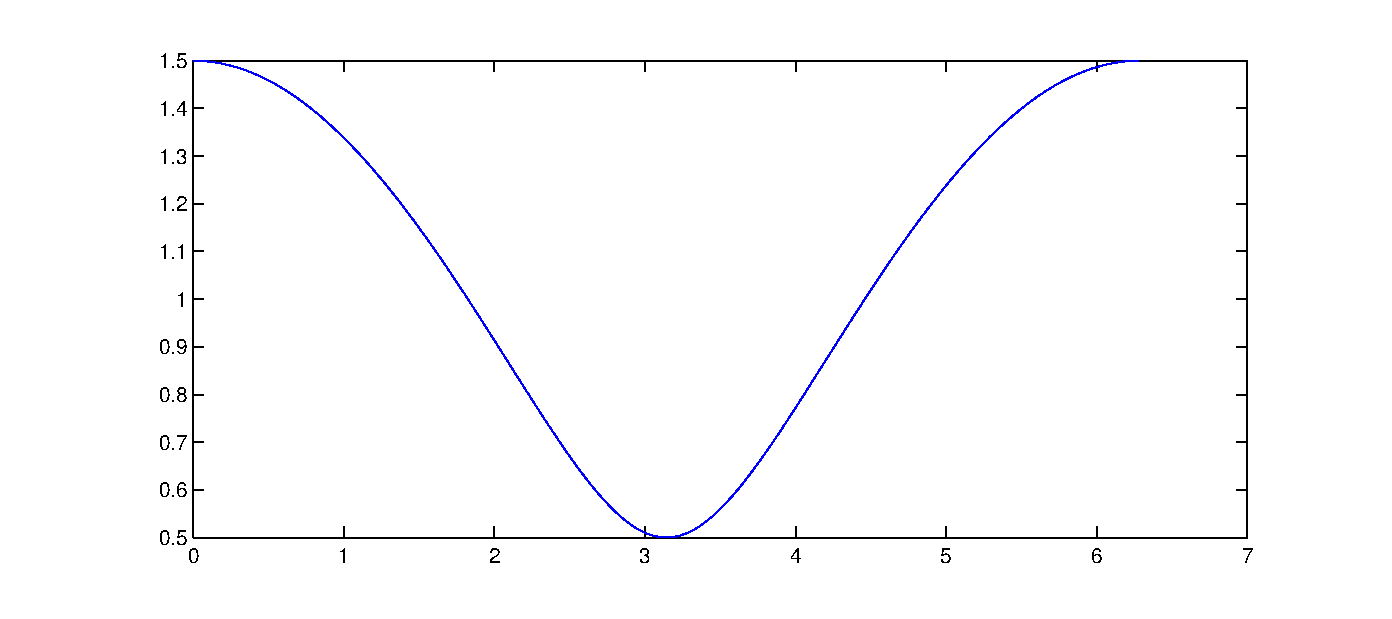
\includegraphics[width=0.4\linewidth]{tp4ex1.eps}
		%	\caption{Normalized received signal}
		%	\label{fig:tp4ex1}
		%\end{figure}	
		
	\item Now that there is a movement, the phase shift is also due to the speed (Doppler shift). So we will use the equation:
	$$ \frac{2\pi}{c}f_c \sin \theta v \Delta t = \frac{2\pi}{\lambda} \sin \theta v \Delta t$$
	Here $\theta = 40^\circ \rightarrow \sin \theta = \frac{\sqrt{2}}{2}$
	
	So $E = E_d + E_d e^{j\frac{2\pi}{\lambda}\frac{\sqrt{2}}{2}v t}$, then, if we compute $E(t_2) - E(t_1) = E e^{j \frac{2\pi}{\lambda} \frac{\sqrt{2}}{2} v t_2} (1 - e^{v (t_1 - t_2)}) = E e^{j \frac{2\pi}{\lambda} \frac{\sqrt{2}}{2}v t_2}(1 - e^{\Delta d})$.
	Then, after normalization, we obtain:
	$$E_n = (1 - e^{\Delta d})$$
	
	\end{enumerate} 
\end{solution}

\begin{solution}
	\begin{enumerate}
		\item We know that the path loss is defined as $P = \frac{4\pi r}{\lambda}^2$ with d the distance, then, if we want a maximal attenuation of $140dB = 1\expten{-14} W$, we can simply replace the variables and retrieve:
		$d_{900} = 265258m$, $d_{1800} = 132629m$
		
		\item If we use the log-normal distribution (corresponding to the shadowing distribution), we can recover $P(X \leq x) = 0.95 = 0.5 erfc(\frac{x - \mu}{\sigma \sqrt{2}}) \rightarrow X = 1.25$. Then we have to "de-normalize" it via: $X = \frac{x - \mu}{\sqrt{2} \sigma}$ so $\mu = x - X\sqrt{2}\sigma = 140 - 1.25\sqrt{2}6 = 129.4dB$.
		So the new distances are: $d_{new~900} = 247553m$, $d_{new~1800} = 123776m$.
		
		At the exercise session, we found something really smaller than before. I think the assistant forgot to convert $\mu$ fro dB to Watts. \notsure
	\end{enumerate}
\end{solution}

\begin{solution}
	\begin{enumerate}
		\item $E_t = s_1(t) + s_2(t) = e^{j\frac{2 \pi}{\lambda} v t}(1 + e^{jk \Delta t})$
		\item The Fourier transform will be two Diracs, a big one and then the second path one (smaller).
		\item TODO \notsure
 		\item TODO
		\item TODO
	\end{enumerate}
\end{solution}
